\documentclass[10pt, aspectratio=169, handout]{beamer}
\usefonttheme{professionalfonts}
%\usetheme{CambridgeUS}
%
% Choose how your presentation looks.
%
% For more themes, color themes and font themes, see:
% http://deic.uab.es/~iblanes/beamer_gallery/index_by_theme.html
%
\mode<presentation>
{
  \usetheme{Berkeley}      % or try Darmstadt, Madrid, Warsaw, ...
  \usecolortheme{beaver} % or try albatross, beaver, crane, ...
  \usefonttheme{default}  % or try serif, structurebold, ...
  \setbeamertemplate{navigation symbols}{}
  \setbeamertemplate{caption}[numbered]
} 

\setbeamertemplate{footline}{%
  \leavevmode%
  \hbox{%
    \begin{beamercolorbox}[wd=.85\paperwidth,ht=2.5ex,dp=1ex,left]{author in head/foot}%
      \usebeamerfont{author in head/foot}Digital Signal Processing, Fall 2025%
    \end{beamercolorbox}%
    \begin{beamercolorbox}[wd=.15\paperwidth,ht=2.5ex,dp=1ex,right]{date in head/foot}%
      \hspace*{0.5em}\insertframenumber{} / \inserttotalframenumber\hspace*{0.5em}%
    \end{beamercolorbox}%
  }%
  \vskip0pt%
}

\usepackage[english]{babel}
\usepackage[utf8x]{inputenc}
\usepackage{tikz}
\usepackage{pgfplots}
\usepackage{array}  % for table column M
\usepackage{makecell} % to break line within a cell
\usepackage{verbatim}
\usepackage{graphicx}
\usepackage{subcaption}
\usepackage{amsfonts}
\usepackage{amsmath}
\usepackage{bm}
\usepackage{epstopdf}
\captionsetup{compatibility=false}
%\usepackage{dsfont}
\usepackage[absolute,overlay]{textpos}
\usetikzlibrary{calc}
\usetikzlibrary{pgfplots.fillbetween, backgrounds}
\usetikzlibrary{positioning}

\usetikzlibrary{pgfplots.groupplots}
\usetikzlibrary{plotmarks}
\usetikzlibrary{calc}

\usepgfplotslibrary{groupplots}
\pgfplotsset{compat=newest} 
%\pgfplotsset{plot coordinates/math parser=false}

\usepackage{hyperref}
\hypersetup{
    colorlinks=true,
    linkcolor=blue,
    filecolor=magenta,      
    urlcolor=cyan,
}

% %% 
% \input{header.tex}

% %%
\title[ECEN 463/863]{Frequency Domain Representation of Discrete Systems}
\author{Maxx Seminario}
\institute{University of Nebraska-Lincoln}
\date{September 27, 2025}

\begin{document}
\begin{frame}
  \titlepage
\end{frame}

\section{Introduction}

% \begin{frame}{Frequency-Domain Representation}
% \begin{center}
% {\Large Digital Signal Processing}\\
% \vspace{0.5cm}
% {\large Frequency-Domain Representation of\\Discrete-Time Signals and Systems}\\
% \vspace{1cm}
% Maxx Seminario\\
% Fall 2025
% \end{center}
% \end{frame}

\begin{frame}{Introduction to Frequency-Domain Analysis}
\begin{itemize}
    \item \textbf{Multiple Signal Representations}:
    \begin{itemize}
        \item Time-domain: Weighted sum of delayed impulses
        \item Frequency-domain: Weighted sum of sinusoids/complex exponentials
    \end{itemize}
    
    \item \textbf{Why Complex Exponentials?}
    \begin{itemize}
        \item Complex exponentials are \textit{eigenfunctions} of LTI systems
        \item Input: $e^{j\omega n}$ → Output: $H(e^{j\omega})e^{j\omega n}$
        \item Sinusoidal input → Sinusoidal output (same frequency)
    \end{itemize}
    
    \item \textbf{Fundamental Property}:
    \begin{itemize}
        \item LTI systems preserve frequency of sinusoidal inputs
        \item Only amplitude and phase change
        \item Changes determined by system's frequency response
    \end{itemize}
    
    % \item \textbf{Practical Importance}:
    % \begin{itemize}
    %     \item Foundation for filter design
    %     \item Spectral analysis of signals
    %     \item System analysis and design
    % \end{itemize}
\end{itemize}
\end{frame}

\begin{frame}{Review: Eigenfunctions and Eigenvalues}
    \textbf{Definition}: For a linear operator $\mathcal{T}$, a function $\phi(t)$ is an \textbf{eigenfunction} if:
    \[
        \mathcal{T}\{\phi(t)\} = \lambda \phi(t)
    \]
    where $\lambda$ is the corresponding \textbf{eigenvalue}.

    \vspace{0.3cm}
    \textbf{Key Properties}:
    \begin{itemize}
        \item Operator transforms eigenfunction into a scaled version of itself
        \item Shape is preserved, only amplitude changes
        \item Eigenvalue $\lambda$ determines the scaling factor
    \end{itemize}

    % \vspace{0.3cm}
    
    % \textbf{LTI Systems as Linear Operators}:
    % \begin{itemize}
    %     \item Convolution is a linear operation: $\mathcal{T}\{x[n]\} = \sum_{k} h[k]x[n-k]$
    %     \item For $x[n] = e^{j\omega n}$: $\mathcal{T}\{e^{j\omega n}\} = H(e^{j\omega}) \cdot e^{j\omega n}$
    %     \item \textbf{Eigenfunction}: $e^{j\omega n}$ (complex exponential)
    %     \item \textbf{Eigenvalue}: $H(e^{j\omega})$ (frequency response)
    % \end{itemize}

    % \vspace{0.3cm}
    \textbf{Why This Matters}: 
    \begin{itemize}
        \item Transform complicated operations into simple scaling
        \item Solving differential/difference equations becomes algebraic
    \end{itemize}
    
   
\end{frame}

\begin{frame}{Eigenfunctions for LTI Systems}
    \textbf{Key Concept}: Complex exponentials are eigenfunctions of LTI systems.

    \vspace{0.3cm}
    \textbf{Input-Output Relation}:
    \[
        y[n] = \sum_{k=-\infty}^{\infty} h[k]e^{j\omega(n-k)} = e^{j\omega n}\sum_{k=-\infty}^{\infty} h[k]e^{-j\omega k} = H(e^{j\omega})e^{j\omega n}
    \]

    % \vspace{0.3cm}
    % \textbf{Frequency Response}:
    % \[
    %     H(e^{j\omega}) = \sum_{k=-\infty}^{\infty} h[k]e^{-j\omega k}
    % \]

    \vspace{0.3cm}
    \textbf{Interpretation}:
    \begin{itemize}
        \item $e^{j\omega n}$ is an \textbf{eigenfunction}
        \item $H(e^{j\omega})$ is the corresponding \textbf{eigenvalue}
        \item $H(e^{j\omega})$ describes amplitude/phase change as function of frequency
    \end{itemize}

    \vspace{0.3cm}
    \textbf{Complex Representation}:
    \[
        H(e^{j\omega}) = H_R(e^{j\omega}) + jH_I(e^{j\omega}) = |H(e^{j\omega})|e^{j\angle H(e^{j\omega})}
    \]
\end{frame}

\section{Ideal Delay}

\begin{frame}{Example 1: Ideal Delay System}
\textbf{System Definition}:
\[
    y[n] = x[n - n_d]
\]
where $n_d$ is a fixed integer delay.

\vspace{0.3cm}
\textbf{Method 1 - Direct Substitution}:
For input $x[n] = e^{j\omega n}$:
\[
    y[n] = e^{j\omega(n-n_d)} = e^{-j\omega n_d} \cdot e^{j\omega n}
\]

Therefore: $H(e^{j\omega}) = e^{-j\omega n_d}$

\vspace{0.3cm}
\textbf{Method 2 - Using Impulse Response}:
Impulse response: $h[n] = \delta[n - n_d]$
\[
    H(e^{j\omega}) = \sum_{n=-\infty}^{\infty} \delta[n-n_d]e^{-j\omega n} = e^{-j\omega n_d}
\]
\end{frame}

\begin{frame}{Example 1: Ideal Delay Analysis}
\textbf{Frequency Response}: $H(e^{j\omega}) = e^{-j\omega n_d} = \cos(\omega n_d) - j\sin(\omega n_d)$

\vspace{0.3cm}
\textbf{Real and Imaginary Parts}:
\begin{align}
    H_R(e^{j\omega}) &= \cos(\omega n_d) \\
    H_I(e^{j\omega}) &= -\sin(\omega n_d)
\end{align}

\vspace{0.3cm}
\textbf{Magnitude and Phase}:
\begin{align}
    |H(e^{j\omega})| &= 1 \\
    \angle H(e^{j\omega}) &= -\omega n_d
\end{align}

\vspace{0.3cm}
\textbf{Interpretation}:
\begin{itemize}
    \item \textbf{Magnitude = 1}: No amplitude change at any frequency
    \item \textbf{Phase = $-\omega n_d$}: Linear phase (pure delay)
    % \item \textbf{Group delay}: $-\frac{d}{d\omega}(-\omega n_d) = n_d$ samples
\end{itemize}
\end{frame}

\section{Superposition Principle}

\begin{frame}{Superposition Principle}
\textbf{Signal Representation}:
If we can represent a signal as:
\[
    x[n] = \sum_k \alpha_k e^{j\omega_k n}
\]

% \vspace{0.3cm}
\textbf{System Output}:
By linearity and the eigenfunction property:
\[
    y[n] = \sum_k \alpha_k H(e^{j\omega_k}) e^{j\omega_k n}
\]

% \vspace{0.3cm}
\textbf{Key Insight}:
\begin{itemize}
    \item Each frequency component is processed independently
    \item System acts as a "filter" for different frequencies
    \item Only need to know $H(e^{j\omega})$ at frequencies $\omega_k$
\end{itemize}

\vspace{0.3cm}
\textbf{This is the foundation for}:
\begin{itemize}
    \item Fourier analysis
    \item Filter design
    \item Spectral analysis
\end{itemize}
\end{frame}

\begin{frame}{Example 2: Sinusoidal Response}
\textbf{Input}: $x[n] = A\cos(\omega_0 n + \phi)$

\vspace{0.3cm}
\textbf{Step 1 - Express using complex exponentials}:
\[
    x[n] = \frac{A}{2}e^{j\phi}e^{j\omega_0 n} + \frac{A}{2}e^{-j\phi}e^{-j\omega_0 n}
\]

\vspace{0.3cm}
\textbf{Step 2 - Apply superposition}:
\begin{align}
    y_1[n] &= H(e^{j\omega_0}) \frac{A}{2}e^{j\phi}e^{j\omega_0 n} \\
    y_2[n] &= H(e^{-j\omega_0}) \frac{A}{2}e^{-j\phi}e^{-j\omega_0 n}
\end{align}

\vspace{0.3cm}
\textbf{Step 3 - Total response}:
\[
    y[n] = \frac{A}{2}\left[H(e^{j\omega_0})e^{j\phi}e^{j\omega_0 n} + H(e^{-j\omega_0})e^{-j\phi}e^{-j\omega_0 n}\right]
\]
\end{frame}

% \begin{frame}{Example 2: Where Does $\theta$ Come From?}
%     \textbf{Starting from the total response}:
%     \[
%         y[n] = \frac{A}{2}\left[H(e^{j\omega_0})e^{j\phi}e^{j\omega_0 n} + H(e^{-j\omega_0})e^{-j\phi}e^{-j\omega_0 n}\right]
%     \]

%     \vspace{0.3cm}
%     \textbf{Step 1}: For real $h[n]$, we have $H(e^{-j\omega_0}) = H^*(e^{j\omega_0})$

%     \vspace{0.3cm}
%     \textbf{Step 2}: Express $H(e^{j\omega_0})$ in polar form:
%     \[
%         H(e^{j\omega_0}) = |H(e^{j\omega_0})|e^{j\theta}
%     \]
%     where $\theta = \angle H(e^{j\omega_0})$

%     \vspace{0.3cm}
%     \textbf{Step 3}: Substitute into the response:
%     \begin{align}
%         y[n] &= \frac{A}{2}\left[|H(e^{j\omega_0})|e^{j\theta}e^{j\phi}e^{j\omega_0 n} + |H(e^{j\omega_0})|e^{-j\theta}e^{-j\phi}e^{-j\omega_0 n}\right] \\
%         &= \frac{A|H(e^{j\omega_0})|}{2}\left[e^{j(\omega_0 n + \phi + \theta)} + e^{-j(\omega_0 n + \phi + \theta)}\right]
%     \end{align}

%     \vspace{0.3cm}
%     \textbf{Step 4}: Use Euler's formula:
%     \[
%         e^{j\alpha} + e^{-j\alpha} = 2\cos(\alpha)
%     \]

%     \vspace{0.3cm}
%     \textbf{Final Result}:
%     \[
%         y[n] = A|H(e^{j\omega_0})|\cos(\omega_0 n + \phi + \theta)
%     \]

%     \textbf{Therefore}: $\theta = \angle H(e^{j\omega_0})$ is the \textbf{phase of the frequency response}
% \end{frame}

\begin{frame}{Example 2: Final Result}
    \textbf{For real impulse response}: $H(e^{-j\omega_0}) = H^*(e^{j\omega_0})$

    \vspace{0.3cm}
    \textbf{Simplified output}:
    \[
        y[n] = A|H(e^{j\omega_0})|\cos(\omega_0 n + \phi + \theta)
    \]
    where $\theta = \angle H(e^{j\omega_0})$

    \vspace{0.3cm}
    \textbf{Key Results}:
    \begin{itemize}
        \item \textbf{Frequency preserved}: Output has same frequency $\omega_0$
        \item \textbf{Amplitude scaled}: By factor $|H(e^{j\omega_0})|$
        \item \textbf{Phase shifted}: By angle $\theta = \angle H(e^{j\omega_0})$
    \end{itemize}

    % \vspace{0.3cm}
    % \textbf{Example - Ideal Delay}:
    % $|H(e^{j\omega_0})| = 1$, $\theta = -\omega_0 n_d$
    % \[
    %     y[n] = A\cos(\omega_0 n + \phi - \omega_0 n_d) = A\cos[\omega_0(n-n_d) + \phi]
    % \]
    % This confirms our intuition: pure delay with no distortion.
\end{frame}


\section{Periodicity in Frequency Domain}

\begin{frame}{Periodicity of Frequency Response}
    \textbf{Fundamental Property}: $H(e^{j\omega})$ is periodic with period $2\pi$.

    \vspace{0.3cm}
    \textbf{Proof}:
    \[
        H(e^{j(\omega+2\pi)}) = \sum_{n=-\infty}^{\infty} h[n]e^{-j(\omega+2\pi)n}
    \]

    Since $e^{-j2\pi n} = 1$ for integer $n$:
    \[
        e^{-j(\omega+2\pi)n} = e^{-j\omega n}e^{-j2\pi n} = e^{-j\omega n}
    \]

    Therefore: $H(e^{j(\omega+2\pi)}) = H(e^{j\omega})$

    \vspace{0.3cm}
    \textbf{Why this occurs}:
    \begin{itemize}
        \item Sequences $\{e^{j\omega n}\}$ and $\{e^{j(\omega+2\pi)n}\}$ are identical (in discrete time!)
        \item System must respond identically to identical inputs
        \item Frequencies $\omega$ and $\omega + 2\pi$ are indistinguishable
    \end{itemize}
\end{frame}

\begin{frame}{Frequency Response Specification}
    \textbf{Key Consequence}: Only need to specify $H(e^{j\omega})$ over one period!

    \vspace{0.3cm}
    \textbf{Common Choices}:
    \begin{itemize}
        \item $0 \leq \omega \leq 2\pi$
        \item $-\pi < \omega \leq \pi$ (most common)
    \end{itemize}

    \vspace{0.3cm}
    \textbf{Frequency Interpretation}:
    \begin{itemize}
        \item \textbf{Low frequencies}: Close to $\omega = 0$ (or even multiples of $\pi$)
        \item \textbf{High frequencies}: Close to $\omega = \pm\pi$ (or odd multiples of $\pi$)
    \end{itemize}

    \vspace{0.3cm}
    \textbf{Important Note}:
    \begin{itemize}
        \item This is different from continuous-time systems
        \item Continuous-time: $H(j\Omega)$ defined for all $\Omega$
        \item Discrete-time: $H(e^{j\omega})$ periodic with period $2\pi$
        \item Digital frequency $\omega$ is normalized (radians per sample)
    \end{itemize}
\end{frame}

\begin{frame}{Ideal Frequency-Selective Filters}
    \textbf{Ideal Lowpass Filter}:
    \begin{center}
    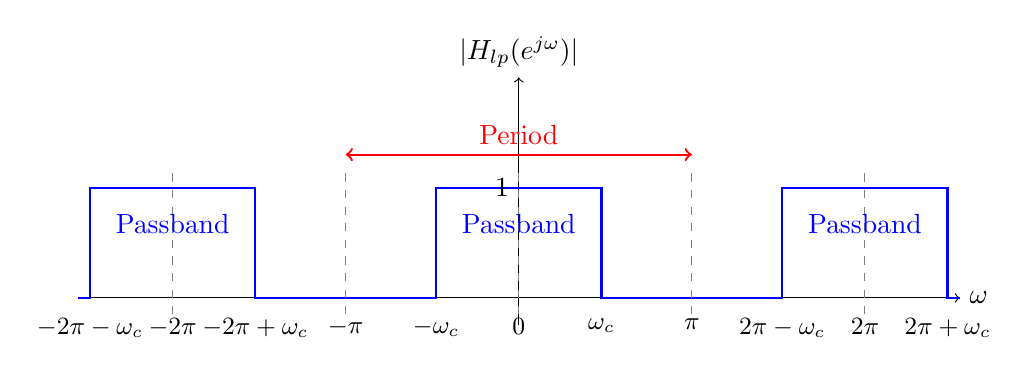
\begin{tikzpicture}[scale=0.7]
        \draw[->] (-8, 0) -- (8, 0) node[right] {$\omega$};
        \draw[->] (0, -0.5) -- (0, 4) node[above] {$|H_{lp}(e^{j\omega})|$};
        
        % Draw the lowpass response with correct periodicity
        % Period around -2π (from -2π-ωc to -2π+ωc)
        \draw[thick, blue] (-8, 0) -- (-7.78, 0) -- (-7.78, 2) -- (-4.78, 2) -- (-4.78, 0) -- (-3.14, 0);
        
        % Period around 0 (from -ωc to +ωc)  
        \draw[thick, blue] (-3.14, 0) -- (-1.5, 0) -- (-1.5, 2) -- (1.5, 2) -- (1.5, 0) -- (3.14, 0);
        
        % Period around +2π (from 2π-ωc to 2π+ωc)
        \draw[thick, blue] (3.14, 0) -- (4.78, 0) -- (4.78, 2) -- (7.78, 2) -- (7.78, 0) -- (8, 0);
        
        % Vertical dashed lines to show period boundaries
        \draw[dashed, gray] (-6.28, -0.3) -- (-6.28, 2.3);
        \draw[dashed, gray] (-3.14, -0.3) -- (-3.14, 2.3);
        \draw[dashed, gray] (0, -0.3) -- (0, 2.3);
        \draw[dashed, gray] (3.14, -0.3) -- (3.14, 2.3);
        \draw[dashed, gray] (6.28, -0.3) -- (6.28, 2.3);
        
        % Labels
        \node[below, font=\small] at (-7.78, -0.2) {$-2\pi-\omega_c$};
        \node[below, font=\small] at (-6.28, -0.2) {$-2\pi$};
        \node[below, font=\small] at (-4.78, -0.2) {$-2\pi+\omega_c$};
        \node[below, font=\small] at (-3.14, -0.2) {$-\pi$};
        \node[below, font=\small] at (-1.5, -0.2) {$-\omega_c$};
        \node[below, font=\small] at (0, -0.2) {$0$};
        \node[below, font=\small] at (1.5, -0.2) {$\omega_c$};
        \node[below, font=\small] at (3.14, -0.2) {$\pi$};
        \node[below, font=\small] at (4.78, -0.2) {$2\pi-\omega_c$};
        \node[below, font=\small] at (6.28, -0.2) {$2\pi$};
        \node[below, font=\small] at (7.78, -0.2) {$2\pi+\omega_c$};
        \node[left] at (0, 2) {$1$};
        
        % Period labels
        % \node[above, red] at (-6.28, 2.4) {Period};
        \node[above, red] at (0, 2.6) {Period};
        % \node[above, red] at (6.28, 2.4) {Period};
        
        % Arrows showing repetition
        % \draw[<->, red, thick] (-6.28, 2.6) -- (0, 2.6);
        \draw[<->, red, thick] (-3.14, 2.6) -- (3.14, 2.6);
        
        % \node[red] at (0, 3) {$2\pi$ periods};
        
        % Add passband labels
        \node[blue, above] at (0, 1) {Passband};
        \node[blue, above] at (-6.28, 1) {Passband};
        \node[blue, above] at (6.28, 1) {Passband};
    \end{tikzpicture}
    \end{center}

    \textbf{Properties}:
    \begin{itemize}
        \item Passbands: $|\omega - 2\pi k| \leq \omega_c$ for integer $k$
        % \item Stopbands: $\omega_c < |\omega - 2\pi k| \leq \pi$ for integer $k$
        \item \textbf{Periodic with period $2\pi$}: $H(e^{j(\omega+2\pi)}) = H(e^{j\omega})$
        \item Each period has identical rectangular passband around multiples of $2\pi$
    \end{itemize}
\end{frame}

\begin{frame}{Other Ideal Filters}
\begin{center}
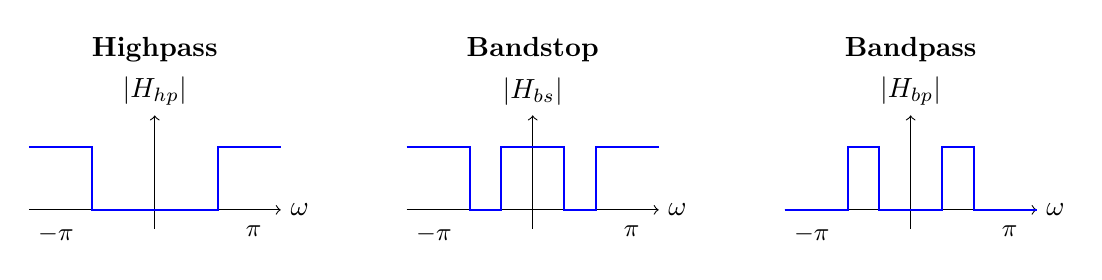
\begin{tikzpicture}[scale=0.8]
    % Highpass filter
    \begin{scope}[shift={(-6,2)}]
        \draw[->] (-2, 0) -- (2, 0) node[right] {$\omega$};
        \draw[->] (0, -0.3) -- (0, 1.5) node[above] {$|H_{hp}|$};
        \draw[thick, blue] (-2, 1) -- (-1, 1) -- (-1, 0) -- (1, 0) -- (1, 1) -- (2, 1);
        \node[below, font=\small] at (-1.57, -0.1) {$-\pi$};
        % \node[below, font=\tiny] at (-1, -0.1) {$-\omega_c$};
        % \node[below, font=\tiny] at (1, -0.1) {$\omega_c$};
        \node[below, font=\small] at (1.57, -0.1) {$\pi$};
        \node[above] at (0, 2.2) {\textbf{Highpass}};
    \end{scope}
    
    % Bandstop filter
    \begin{scope}[shift={(0,2)}]
        \draw[->] (-2, 0) -- (2, 0) node[right] {$\omega$};
        \draw[->] (0, -0.3) -- (0, 1.5) node[above] {$|H_{bs}|$};
        \draw[thick, blue] (-2, 1) -- (-1, 1) -- (-1, 0) -- (-0.5, 0) -- (-0.5, 1) -- (0.5, 1) -- (0.5, 0) -- (1, 0) -- (1, 1) -- (2, 1);
        % \node[below, font=\tiny] at (-1, -0.1) {$-\omega_b$};
        % \node[below, font=\tiny] at (-0.5, -0.1) {$-\omega_a$};
        % \node[below, font=\tiny] at (0.5, -0.1) {$\omega_a$};
        % \node[below, font=\tiny] at (1, -0.1) {$\omega_b$};
        \node[below, font=\small] at (-1.57, -0.1) {$-\pi$};
        \node[below, font=\small] at (1.57, -0.1) {$\pi$};
        \node[above] at (0, 2.2) {\textbf{Bandstop}};
    \end{scope}
    
    % Bandpass filter
    \begin{scope}[shift={(6,2)}]
        \draw[->] (-2, 0) -- (2, 0) node[right] {$\omega$};
        \draw[->] (0, -0.3) -- (0, 1.5) node[above] {$|H_{bp}|$};
        \draw[thick, blue] (-2, 0) -- (-1, 0) -- (-1, 1) -- (-0.5, 1) -- (-0.5, 0) -- (0.5, 0) -- (0.5, 1) -- (1, 1) -- (1, 0) -- (2, 0);
        % \node[below, font=\tiny] at (-1, -0.1) {$-\omega_b$};
        % \node[below, font=\tiny] at (-0.5, -0.1) {$-\omega_a$};
        % \node[below, font=\tiny] at (0.5, -0.1) {$\omega_a$};
        % \node[below, font=\tiny] at (1, -0.1) {$\omega_b$};
        \node[below, font=\small] at (-1.57, -0.1) {$-\pi$};
        \node[below, font=\small] at (1.57, -0.1) {$\pi$};
        \node[above] at (0, 2.2) {\textbf{Bandpass}};
    \end{scope}
\end{tikzpicture}
\end{center}

\textbf{Filter Types}:
\begin{itemize}
    \item \textbf{Highpass}: Passes high frequencies, rejects low frequencies
    \item \textbf{Bandstop (Notch)}: Rejects frequencies in a band
    \item \textbf{Bandpass}: Passes frequencies in a band, rejects others
\end{itemize}

\textbf{Note}: All responses are periodic with period $2\pi$
\end{frame}

\section{Moving Average System}

\begin{frame}{Example 3: Moving Average System}
    \textbf{System Definition} (causal, $M_1 = 0$):
    \[
        h[n] = \begin{cases}
            \frac{1}{M_2+1}, & 0 \leq n \leq M_2 \\
            0, & \text{otherwise}
        \end{cases}
    \]

    % \vspace{0.3cm}
    \textbf{Frequency Response}:
    \[
        H(e^{j\omega}) = \frac{1}{M_2+1} \sum_{n=0}^{M_2} e^{-j\omega n}
    \]

    % \vspace{0.3cm}
    \textbf{Using Geometric Series Formula}:
    \[
        H(e^{j\omega}) = \frac{1}{M_2+1} \frac{1-e^{-j\omega(M_2+1)}}{1-e^{-j\omega}}
    \]

    % \vspace{0.3cm}
    \textbf{Simplified Form}:
    \[
        H(e^{j\omega}) = \frac{1}{M_2+1} \frac{\sin[\omega(M_2+1)/2]}{\sin(\omega/2)} e^{-j\omega M_2/2}
    \]
\end{frame}






\begin{frame}{Moving Average: Frequency Response Analysis}
    \begin{columns}
    % Left column with TikZ plot
    \begin{column}{0.55\textwidth}
        \raisebox{1.5cm}{
            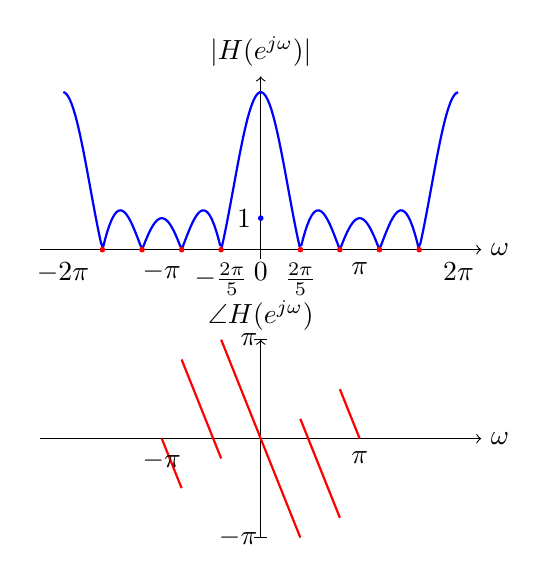
\begin{tikzpicture}[scale=0.4]
                % Magnitude response
                \begin{scope}[shift={(0,3)}]
                    \draw[->] (-7, 0) -- (7, 0) node[right] {$\omega$};
                    \draw[->] (0, -0.3) -- (0, 5.5) node[above] {$|H(e^{j\omega})|$};
                    
                    % Draw approximate sinc-like response with scaled amplitude
                    \draw[thick, blue, domain=-6.27:6.27, samples=200] plot (\x, {
                        abs(\x) < 0.01 ? 1.0 : 1.0*abs(sin(5*\x*180/3.14/2)/(sin(\x*180/3.14/2) + 0.000001))
                    });
                    
                    % Mark the value at ω = 0 explicitly
                    \filldraw[blue] (0, 1.0) circle (2pt);
                    
                    \node[below] at (-1.26, -0.1) {$-\frac{2\pi}{5}$};
                    \node[below] at (1.26, -0.1) {$\frac{2\pi}{5}$};
                    \node[below] at (-6.28, -0.1) {$-2\pi$};
                    \node[below] at (-3.14, -0.1) {$-\pi$};
                    \node[below] at (0, -0.1) {$0$};
                    \node[below] at (3.14, -0.1) {$\pi$};
                    \node[below] at (6.28, -0.1) {$2\pi$};
                    \node[left] at (0, 1.0) {$1$};
                    
                    % Mark nulls
                    \foreach \x in {-5.03,-3.77,-2.51,-1.26,1.26,2.51,3.77,5.03} {
                        \filldraw[red] (\x, 0) circle (2pt);
                    }
                \end{scope}
                
                % Phase response - scaled to -π to π
                \begin{scope}[shift={(0,-3)}]
                    \draw[->] (-7, 0) -- (7, 0) node[right] {$\omega$};
                    % Set y-axis from -π to π
                    \draw[->] (0, -3.14) -- (0, 3.14) node[above] {$\angle H(e^{j\omega})$};

                    \draw (-0.2, pi) -- (0.2, pi) node[left] {$\pi$};
                    \draw (-0.2, -pi) -- (0.2, -pi) node[left] {$-\pi$};
                    
                    \draw[thick, red] (-2*pi/5, pi) -- (2*pi/5, -pi);
                    \draw[thick, red] (-4*pi/5, 4*pi/5) -- (-2*pi/5, -pi/5);
                    \draw[thick, red] (2*pi/5, pi/5) -- (4*pi/5, -4*pi/5);
                    \draw[thick, red] (4*pi/5, pi/2) -- (pi, 0);
                    \draw[thick, red] (-pi, 0) -- (-4*pi/5, -pi/2);

                    % Labels for key frequencies
                    % \node[below] at (-2.51, -0.1) {$-\frac{4\pi}{5}$};
                    % \node[below] at (2.51, -0.1) {$\frac{4\pi}{5}$};
                    % \node[below] at (-1.25, -0.1) {$-\frac{2\pi}{5}$};
                    % \node[below] at (1.25, -0.1) {$\frac{2\pi}{5}$};
                    \node[below] at (-pi, -0.1) {$-\pi$};
                    \node[below] at (pi, -0.1) {$\pi$};
                \end{scope}
            \end{tikzpicture}
        }
    \end{column}

        % Right column with text
        \begin{column}{0.45\textwidth}
            \textbf{For $M_1 = 0, M_2 = 4$}:
            
            \medskip
            
            \textbf{Key Observations}:
            \begin{itemize}
                \item \textbf{Lowpass character}: Attenuates high frequencies
                \item \textbf{Linear phase}: $\angle H(e^{j\omega}) = -2\omega \bmod \frac{2\pi}{5}$
                \item \textbf{Phase jumps}: At frequencies where $\sin(5\omega/2) = 0$
            \end{itemize}
        \end{column}
    \end{columns}
\end{frame}





\begin{frame}{Moving Average: Physical Interpretation}
\textbf{Why does it act like a lowpass filter?}

\vspace{0.3cm}
\textbf{Time Domain View}:
\[
    y[n] = \frac{1}{M_2+1} \sum_{k=0}^{M_2} x[n-k]
\]

\begin{itemize}
    \item Averages $(M_2+1)$ consecutive samples
    \item Rapid variations (high frequencies) tend to cancel out
    \item Slow variations (low frequencies) are preserved
    \item Smoothing effect on the input signal
\end{itemize}

\vspace{0.3cm}
\textbf{Frequency Domain Confirmation}:
\begin{itemize}
    \item $|H(e^{j\omega})|$ maximum at $\omega = 0$ (DC)
    \item $|H(e^{j\omega})|$ decreases as $\omega$ increases
    \item First zero at $\omega = \frac{2\pi}{M_2+1}$
    \item Higher frequencies are attenuated
\end{itemize}

% \vspace{0.3cm}
% \textbf{Design Parameter}:
% \begin{itemize}
%     \item Larger $M_2$ → More averaging → Better lowpass filtering
%     \item Trade-off: More delay and computation
% \end{itemize}
\end{frame}

\section{Summary}

\begin{frame}{Summary: Key Concepts}
\begin{itemize}
    \item \textbf{Eigenfunction Property}:
    \[
        e^{j\omega n} \rightarrow H(e^{j\omega})e^{j\omega n}
    \]
    
    \item \textbf{Frequency Response}:
    \[
        H(e^{j\omega}) = \sum_{k=-\infty}^{\infty} h[k]e^{-j\omega k}
    \]
    
    \item \textbf{Periodicity}: $H(e^{j(\omega+2\pi)}) = H(e^{j\omega})$
    
    \item \textbf{Sinusoidal Response}:
    \[
        A\cos(\omega_0 n + \phi) \rightarrow A|H(e^{j\omega_0})|\cos(\omega_0 n + \phi + \angle H(e^{j\omega_0}))
    \]
    
    \item \textbf{Filter Design}: Use $H(e^{j\omega})$ to shape frequency content
    
    \item \textbf{System Analysis}: Frequency response reveals system behavior
\end{itemize}

\vspace{0.3cm}
\textbf{Next Topics}: Discrete-Time Fourier Transform (DTFT), Z-Transform
\end{frame}


\end{document}
